%% abtex2-modelo-trabalho-academico.tex, v-1.9.2 laurocesar
%% Copyright 2012-2014 by abnTeX2 group at http://abntex2.googlecode.com/ 
%%
%% This work may be distributed and/or modified under the
%% conditions of the LaTeX Project Public License, either version 1.3
%% of this license or (at your option) any later version.
%% The latest version of this license is in
%%   http://www.latex-project.org/lppl.txt
%% and version 1.3 or later is part of all distributions of LaTeX
%% version 2005/12/01 or later.
%%
%% This work has the LPPL maintenance status `maintained'.
%% 
%% The Current Maintainer of this work is the abnTeX2 team, led
%% by Lauro César Araujo. Further information are available on 
%% http://abntex2.googlecode.com/
%%
%% This work consists of the files abntex2-modelo-trabalho-academico.tex,
%% abntex2-modelo-include-comandos and abntex2-modelo-references.bib
%%

% ------------------------------------------------------------------------
% ------------------------------------------------------------------------
% abnTeX2: Modelo de Trabalho Academico (tese de doutorado, dissertacao de
% mestrado e trabalhos monograficos em geral) em conformidade com 
% ABNT NBR 14724:2011: Informacao e documentacao - Trabalhos academicos -
% Apresentacao
% ------------------------------------------------------------------------
% ------------------------------------------------------------------------

\documentclass[
	% -- opções da classe memoir --
	12pt,				% tamanho da fonte
	openright,			% capítulos começam em pág ímpar (insere página vazia caso preciso)
	twoside,			% para impressão em verso e anverso. Oposto a oneside
	a4paper,			% tamanho do papel. 
	% -- opções da classe abntex2 --
	%chapter=TITLE,		% títulos de capítulos convertidos em letras maiúsculas
	%section=TITLE,		% títulos de seções convertidos em letras maiúsculas
	%subsection=TITLE,	% títulos de subseções convertidos em letras maiúsculas
	%subsubsection=TITLE,% títulos de subsubseções convertidos em letras maiúsculas
	% -- opções do pacote babel --
	english,			% idioma adicional para hifenização
	french,				% idioma adicional para hifenização
	spanish,			% idioma adicional para hifenização
	brazil				% o último idioma é o principal do documento
	]{abntex2}

% ---
% Pacotes básicos 
% ---
\usepackage{lmodern}			% Usa a fonte Latin Modern			
\usepackage[T1]{fontenc}		% Selecao de codigos de fonte.
\usepackage[utf8]{inputenc}		% Codificacao do documento (conversão automática dos acentos)
\usepackage{lastpage}			% Usado pela Ficha catalográfica
\usepackage{indentfirst}		% Indenta o primeiro parágrafo de cada seção.
\usepackage{color}				% Controle das cores
\usepackage{graphicx}			% Inclusão de gráficos
\usepackage{microtype} 			% para melhorias de justificação
\usepackage{pythonhighlight}
\usepackage{listings}
\usepackage{xcolor}
\usepackage{bm}
% ---
		
% ---
% Pacotes adicionais, usados apenas no âmbito do Modelo Canônico do abnteX2
% ---
\usepackage{lipsum}				% para geração de dummy text
% ---

% ---
% Pacotes de citações
% ---
\usepackage[brazilian,hyperpageref]{backref}	 % Paginas com as citações na bibl
\usepackage[alf]{abntex2cite}	% Citações padrão ABNT

% --- 
% CONFIGURAÇÕES DE PACOTES
% --- 
\lstset{
  basicstyle=\fontsize{11}{13}\selectfont\ttfamily
}
\graphicspath{ {./images/} }
% ---
% Configurações do pacote backref
% Usado sem a opção hyperpageref de backref
\renewcommand{\backrefpagesname}{Citado na(s) página(s):~}
% Texto padrão antes do número das páginas
\renewcommand{\backref}{}
% Define os textos da citação
\renewcommand*{\backrefalt}[4]{
	\ifcase #1 %
		Nenhuma citação no texto.%
	\or
		Citado na página #2.%
	\else
		Citado #1 vezes nas páginas #2.%
	\fi}%
% ---

% ---
% Informações de dados para CAPA e FOLHA DE ROSTO
% ---
\titulo{Relatório}
\autor{Bruno Duarte Barreto Borges\\Fabio Oliveira de Abreu\\Erik Kazuo Sugawara}
\local{Florianópolis, SC}
\data{2021}
\orientador{Alvaro Junio Pereira Franco}
\instituicao{%
  Universidade Federal de Santa Catarina
  \par
  Departamento de Informática e Estatística
  \par
  INE5426 - Construção de Compiladores}
\tipotrabalho{Relatório}
% O preambulo deve conter o tipo do trabalho, o objetivo, 
% o nome da instituição e a área de concentração 
\preambulo{Relatório sobre a Construção de um Compilador, feito 
pelos alunos: Bruno Duarte Barreto Borges, Fabio Oliveira de Abreu e
Erik Kazuo Sugawara. Para obtenção da aprovação na disciplina Construção
de Compiladores, ministrada pelo Prof. Dr. Alvaro Junio Pereira Franco.}
% ---


% ---
% Configurações de aparência do PDF final

% alterando o aspecto da cor azul
\definecolor{blue}{RGB}{41,5,195}

% informações do PDF
\makeatletter
\hypersetup{
     	%pagebackref=true,
		pdftitle={\@title}, 
		pdfauthor={\@author},
    	pdfsubject={\imprimirpreambulo},
	    pdfcreator={LaTeX with abnTeX2},
		pdfkeywords={abnt}{latex}{abntex}{abntex2}{trabalho acadêmico}, 
		colorlinks=true,       		% false: boxed links; true: colored links
    	linkcolor=blue,          	% color of internal links
    	citecolor=blue,        		% color of links to bibliography
    	filecolor=magenta,      		% color of file links
		urlcolor=blue,
		bookmarksdepth=4
}
\makeatother
% --- 

% --- 
% Espaçamentos entre linhas e parágrafos 
% --- 

% O tamanho do parágrafo é dado por:
\setlength{\parindent}{1.3cm}

% Controle do espaçamento entre um parágrafo e outro:
\setlength{\parskip}{0.2cm}  % tente também \onelineskip

% ---
% compila o indice
% ---
\makeindex
% ---

% ----
% Início do documento
% ----
\begin{document}

% Retira espaço extra obsoleto entre as frases.
\frenchspacing 

% ----------------------------------------------------------
% ELEMENTOS PRÉ-TEXTUAIS
% ----------------------------------------------------------
% \pretextual

% ---
% Capa
% ---
\imprimircapa
% ---

% ---
% Folha de rosto
% (o * indica que haverá a ficha bibliográfica)
% ---
\imprimirfolhaderosto*
% ---

% ---
% Inserir a ficha bibliografica
% ---

% Isto é um exemplo de Ficha Catalográfica, ou ``Dados internacionais de
% catalogação-na-publicação''. Você pode utilizar este modelo como referência. 
% Porém, provavelmente a biblioteca da sua universidade lhe fornecerá um PDF
% com a ficha catalográfica definitiva após a defesa do trabalho. Quando estiver
% com o documento, salve-o como PDF no diretório do seu projeto e substitua todo
% o conteúdo de implementação deste arquivo pelo comando abaixo:
%
% \begin{fichacatalografica}
%     \includepdf{fig_ficha_catalografica.pdf}
% \end{fichacatalografica}

% ---
% inserir lista de abreviaturas e siglas
% ---
\begin{siglas}
  \item[PLY] Python Lexx-Yacc
  \item[BNF] Bakus-Naur Form
\end{siglas}
% ---

% ---
% inserir o sumario
% ---
\pdfbookmark[0]{\contentsname}{toc}
\tableofcontents*
\cleardoublepage
% ---



% ----------------------------------------------------------
% ELEMENTOS TEXTUAIS
% ----------------------------------------------------------
\textual

% ----------------------------------------------------------
% Introdução (exemplo de capítulo sem numeração, mas presente no Sumário)
% ----------------------------------------------------------
\chapter*[Introdução]{Introdução}
\addcontentsline{toc}{chapter}{Introdução}
% ----------------------------------------------------------

Um compilador é um programa de sistema que traduz uma linguagem de alto nível
para um programa equivalente em código de máquina para um processador. Sendo assim,
um compilador não produz diretamente o código de máquina, mas sim um programa
semanticamente equivalente na linguagem simbólica (assembly), que é traduzido para o programa em linguagem de máquina através de montadores\footnote{\url{https://www.dca.fee.unicamp.br/cursos/EA876/apostila/HTML/node37.html}}.

Este trabalho, em sua primeira fase, tem como objetivo criar um compilador através de um
analisador léxico e sintático para uma linguagem (AL). Para facilitar os estudos na criação do compilador,
foi disponibilizada a linguagem ``LCC-2021-2'' derivada da gramática ``CC-2021-2''
na forma BNF(Backus-Naur Form), inspirada na gramática X++ de Delamaro
\footnote{\url{http://conteudo.icmc.usp.br/pessoas/delamaro/SlidesCompiladores/
CompiladoresFinal.pdf}}.

As atividades contidas neste relatório foram feitas com a linguagem Python em
conjunto da ferramenta PLY (Python Lex-Yacc)\footnote{\url{https://www.dabeaz.com/ply/}},
uma implementação dos geradores de analisadores léxico e sintático (Lex-Yacc) para Python.
Dessa forma, com o auxílio de ferramentas que permitem gerar analisadores, mostraremos
o funcionamento do analisador léxico através de seu algoritmo e da sua aplicação com 
exemplos de programas em alto nível baseadas na gramática ``CC-2021-2''.




% ----------------------------------------------------------
% PARTE
% ----------------------------------------------------------
\part{Ferramenta}
% ----------------------------------------------------------
\chapter{Python Lex-Yacc}
\section{Sobre a ferramenta}
O PLY é uma implementação pura em Python baseada nas ferramentas de construção
de compiladores lex e yacc. Possui suporte para LARL(1) e mecanismos
de validação, verificação de erros e diagnósticos. Sua primeira versão foi desenvolvida
na Universidade de Chicago, para dar suporte à disciplina Introdução a Compiladores.
A sua versão mais recente é o PLY-4.0, que requer o Python na versão 3.6 ou mais nova. 

Ele consiste em dois módulos separados: o lex.py e o yacc.py. O módulo lex.py é utilizado
para separar as entradas em texto do código em uma coleção de tokens baseadas em suas respectivas 
expressões regulares. O yacc.py é utilizado para reconhecer a sintaxe de uma linguagem 
baseada em uma gramática livre de contexto. Além disso, possui utilidades como verificação
de erros, validação de gramática, suporte para produções vazias, tokens de erros e regras de
precedência para resolver ambiguidades.

\section{Lex}
O Lex é utilizado para realizar a atribuição dos tokens com as entradas (\emph{strings}).
Os nomes dos tokens podem ser declarados de forma simples através de uma lista. Um token
que é identificado se torna um objeto da classe LexToken.
\begin{python}
import ply.lex as lex
import ply.yacc as yacc

# RESERVED WORDS
reserved = [
    'DEF',         # def
    'BREAK',       # break
    'FOR',         # for
    'IF',          # if
    'ELSE',        # else
    'INT',         # int
    'FLOAT',       # float
    'NEW',         # new
    'PRINT',       # print
    'READ',        # read
    'RETURN',      # return
    'STRING',      # string
]
\end{python}

	Dada uma lista de tokens, podemos definir suas expressões regulares, que podem
ser de forma simples ou complexa. Note que por definição da ferramenta,
as expressões regulares são declaradas como uma variável que se inicia com ``t\_'',
seguida pelo nome do token definido na lista. Segue um exemplo das expressões
regulares para tokens simples, como: \emph{Assign, Greater Than, Less Than, Equals, Less Equal,
Greater Equal, Not Equal, Plus, Minus, Multiply, Divide e Rem}.
\\
\begin{python}
t_ASSIGN = r'\='
t_GT = r'\>'
t_LT = r'\<'
t_EQ = r'\=='
t_LE = r'\<='
t_GE = r'\>='
t_NEQ = r'\!='
t_PLUS = r'\+'
t_MINUS = r'\-'
t_MULTIPLY = r'\*'
t_DIVIDE = r'\/'
t_REM = r'\%'
\end{python}

Para tokens que requerem maior complexidade para serem identificados, podemos declará-los através de funções
que também se iniciam pelos caracteres ``t\_'' seguidos pelo nome do token
definido. Note que também podemos realizar o tratamento dos valores obtidos acessando
o atributo \emph{value} do objeto LexToken.
\\
\begin{python}
def t_float_constant(t):
    r'[+-]?\d+\.\d+([eE][+-]?\d+)?'
    t.value = float(t.value)
    return t

def t_int_constant(t):
    r'[+-]?\d+'
    t.value = int(t.value)
    return t

def t_string_constant(t):
    r'"[^"\n\r]*"'
    return t

def t_IDENT(t):
    r'[a-zA-Z_][a-zA-Z_0-9]*'
    return t
\end{python}
\newpage


Com essa ferramenta também podemos fazer tratativas de leitura e identificação de erros.
Ela também segue as definições de nomenclatura para tokens. Seguem alguns exemplos
de tratamento de leitura para ignorar caracteres em branco, fim de linhas e caracteres ilegais.
\begin{python}
t_ignore = r' ' # Ignore spaces between char.

def t_newline(t):
	r'\n+'
	t.lexer.lineno += len(t.value)

def t_error(t):
    errors.append("Illegal char %s in line %d, column %d" % (t.value[0], t.lexer.lineno, find_column(t)))
    t.lexer.skip(1)

\end{python}

Para demonstrar o funcionamento do analisador léxico, executamos o seguinte
código. A saída é um LexToken, onde os atributos correspondem respectivamente ao 
identificador do token, símbolo, linha e coluna.

\begin{python}
# Test it out
data = '''
3 + 4 * 10
'''

# Give the lexer some input
lexer.input(data)

# Tokenize
while True:
    tok = lexer.token()
    if not tok:
        break      # No more input
    print(tok)
\end{python}
\noindent Saída :
\begin{lstlisting}[language=bash]
    LexToken(NUMBER,3,2,1)
    LexToken(PLUS,'+',2,3)
    LexToken(NUMBER,4,2,5)
    LexToken(MULTIPLY,'*',2,7)
    LexToken(NUMBER,10,2,10)

\end{lstlisting}
% ---
% Capitulo com exemplos de comandos inseridos de arquivo externo 
% ---
\include{abntex2-modelo-include-comandos}
% ---

% ----------------------------------------------------------
% PARTE
% ----------------------------------------------------------
\part{Analisador Léxico}
% ----------------------------------------------------------

% ---
% Capitulo de revisão de literatura
% ---
\chapter{Metodologia}
% ---

% ---
\section{Extração dos tokens}
% ---
	Para obter os tokens, utilizamos a gramática ``CC-2021-2'' como base
    e dividimos cada um deles em um dos seguintes grupos: palavras reservadas,
	operadores, símbolos especiais, constantes e identificadores. Além disso,
	alteramos a gramática de modo que seja possível retornar valores com o token ``\emph{return}''.

\begin{python}
# RESERVED WORDS
reserved = [
    'DEF',         # def
    'BREAK',       # break
    'FOR',         # for
    'IF',          # if
    'ELSE',        # else
    'INT',         # int
    'FLOAT',       # float
    'NEW',         # new
    'PRINT',       # print
    'READ',        # read
    'RETURN',      # return
    'STRING',      # string
] 
\end{python}

\begin{python}
# OPERATORS
operators = [
    'ASSIGN',      # =
    'GT',          # >
    'LT',          # <
    'EQ',          # ==
    'LE',          # <=
    'GE',          # >=
    'NEQ',         # !=
    'PLUS',        # +
    'MINUS',       # -
    'MULTIPLY',    # *
    'DIVIDE',      # / 
    'REM'          # %
]
\end{python}
\newpage

\begin{python}
# SPECIAL SYMBOLS
special = [
    'LPAREN',      # (
    'RPAREN',      # )
    'LBRACE',      # {
    'RBRACE',      # }
    'LBRACKET',    # [
    'RBRACKET',    # ]
    'SEMICOLON',   # ;
    'COMMA',       # ,
]
\end{python}

\begin{python}
# CONSTANTS
constant = [
    'int_constant',
    'string_constant',
    'float_constant',
    'null_constant'
]
\end{python}

\begin{python}
# IDENTIFIERS
identifiers = [
    'IDENT'
]
\end{python}

\begin{python}
tokens = reserved + operators + special + constant + identifiers
\end{python}
\section{Expressões Regulares}
Após a identificação dos tokens, criamos a expressão regular de cada um deles.
\begin{python}
t_ignore = r' ' # Ignore spaces between char.

def t_DEF(t):
    r'def'
    return t

def t_BREAK(t):
    r'break'
    return t

def t_FOR(t):
    r'for'
    return t
\end{python}

\begin{python}
def t_IF(t):
    r'if'
    return t

def t_ELSE(t):
    r'else'
    return t

def t_NEW(t):
    r'new'
    return t

def t_PRINT(t):
    r'print'
    return t

def t_READ(t):
    r'read'
    return t

def t_RETURN(t):
    r'return'
    return t

def t_STRING(t):
    r'string'
    return t

def t_INT(t):
    r'int'
    return t

def t_FLOAT(t):
    r'float'
    return t
\end{python}

\begin{python}
def t_null_constant(t):
    r'null'
    return t

def t_float_constant(t):
    r'[+-]?\d+\.\d+([eE][+-]?\d+)?'
    t.value = float(t.value)
    return t
\end{python}
\newpage
\begin{python}
def t_int_constant(t):
    r'[+-]?\d+'
    t.value = int(t.value)
    return t

def t_string_constant(t):
    r'"[^"\n\r]*"'
    return t

def t_IDENT(t):
    r'[a-zA-Z_][a-zA-Z_0-9]*'
    return t

def t_newline(t):
    r'\n+'
    t.lexer.lineno += len(t.value)

errors = []

def t_error(t):
    errors.append("Illegal char %s in line %d, column %d" % (t.value[0], t.lexer.lineno, find_column(t)))
    t.lexer.skip(1)
\end{python}

Além da criação das expressões regulares, também foi criado uma função que imprime 
a tabela de símbolos de forma elegante no terminal.
\\
\begin{python}
def print_table(lexer):
    pattern = "{:^25} | {:^60} | {:^7} | {:^7}"
    print("\033[4m" + pattern.format("TOKEN", "VALUE", "LINE", "COLUMN") + "\033[0m")
    while True:
        tok = lexer.token()
        if not tok:
            break
        print(pattern.format(tok.type, tok.value, tok.lineno, find_column(tok))) 

    for e in errors:
        print(e)

\end{python}
\newpage
\section{Analisador Léxico}
Com os tokens e expressões regulares definidos, executamos o analisador léxico e obtemos
a sua tabela de símbolos formatada através da função ``print\_table''.

\begin{lstlisting}[language=bash]
		$ make run file='tmp/lil_example.lcc'

             TOKEN      |    VALUE    |  LINE   | COLUMN 
              DEF       |     def     |    1    |    1   
             IDENT      | hello_world |    1    |    5   
            LPAREN      |      (      |    1    |   16   
            RPAREN      |      )      |    1    |   17   
            LBRACE      |      {      |    1    |   19   
             PRINT      |    print    |    2    |    5   
        string_constant |"hello world"|    2    |   11   
           SEMICOLON    |      ;      |    2    |   24   
            RBRACE      |      }      |    3    |    1   
              INT       |     int     |    5    |    1   
             IDENT      |      x      |    5    |    5   
           SEMICOLON    |      ;      |    5    |    6   
             IDENT      |      x      |    6    |    1   
            ASSIGN      |      =      |    6    |    3   
         int_constant   |      10     |    6    |    5   
           SEMICOLON    |      ;      |    6    |    7   
              IF        |      if     |    8    |    1   
            LPAREN      |      (      |    8    |    4   
             IDENT      |      x      |    8    |    5   
              GT        |      >      |    8    |    7   
         int_constant   |      30     |    8    |    9   
            RPAREN      |      )      |    8    |   11   
            LBRACE      |      {      |    8    |   13   
             IDENT      | hello_world |    9    |    5   
            LPAREN      |      (      |    9    |   16   
            RPAREN      |      )      |    9    |   17   
           SEMICOLON    |      ;      |    9    |   18   
            RBRACE      |      }      |   10    |    1   
             ELSE       |     else    |   10    |    3   
            LBRACE      |      {      |   10    |    8   
             PRINT      |    print    |   11    |    5   
        string_constant |    "erro"   |   11    |   11   
           SEMICOLON    |      ;      |   11    |   17   
            RBRACE      |      }      |   12    |    1  
\end{lstlisting}


% ----------------------------------------------------------
% PARTE
% ----------------------------------------------------------
% ----------------------------------------------------------

% ---
% primeiro capitulo de Resultados
% ---
\chapter{Diagrama de Transição}
% ---
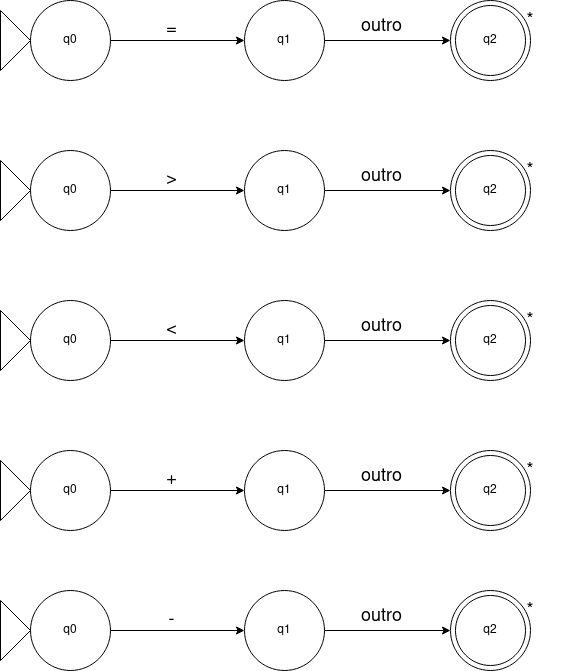
\includegraphics[scale=0.7]{1.png}
\\
\\
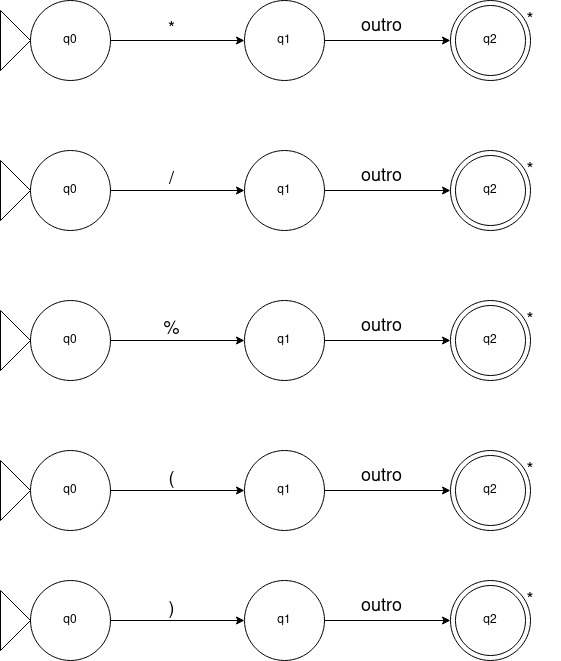
\includegraphics[scale=0.7]{2.png}
\\
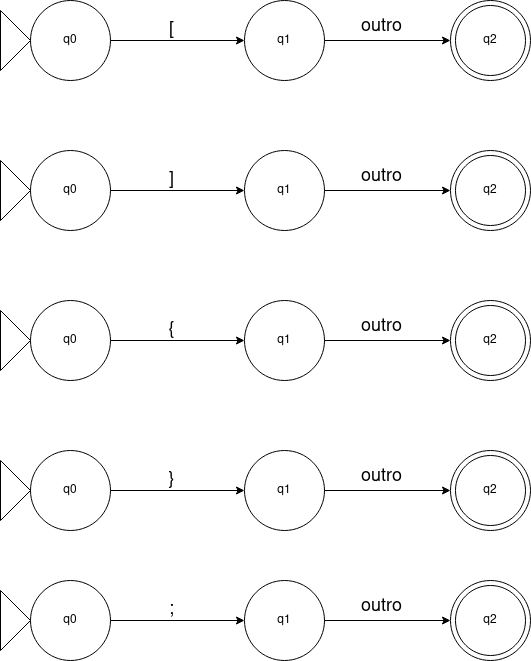
\includegraphics[scale=0.7]{3.png}
\\
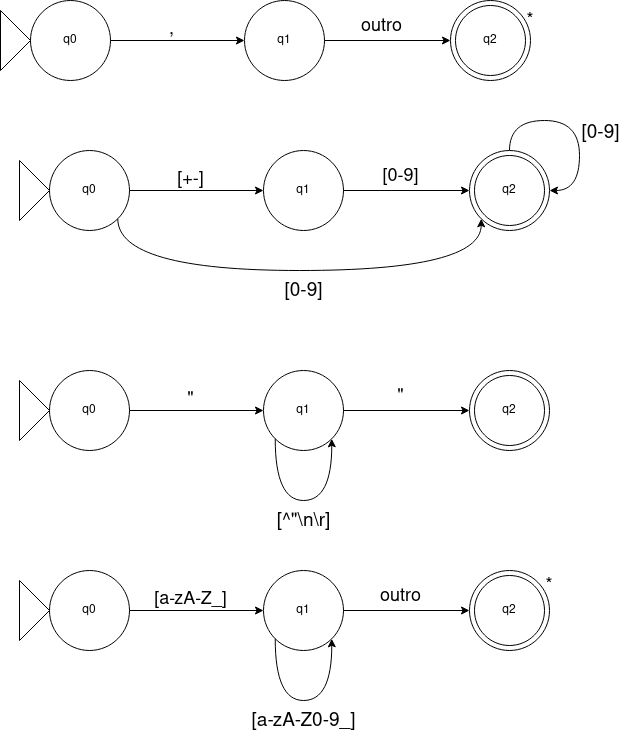
\includegraphics[scale=0.7]{4.png}
\\
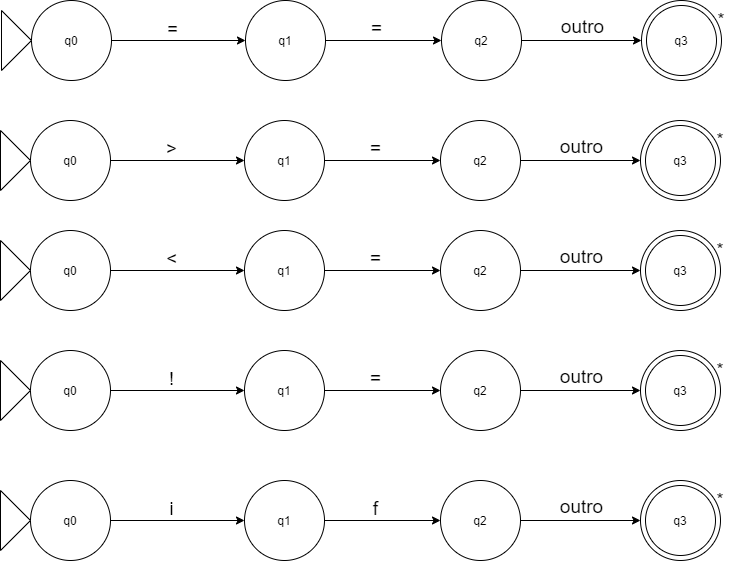
\includegraphics[scale=0.7]{5.png}
\\
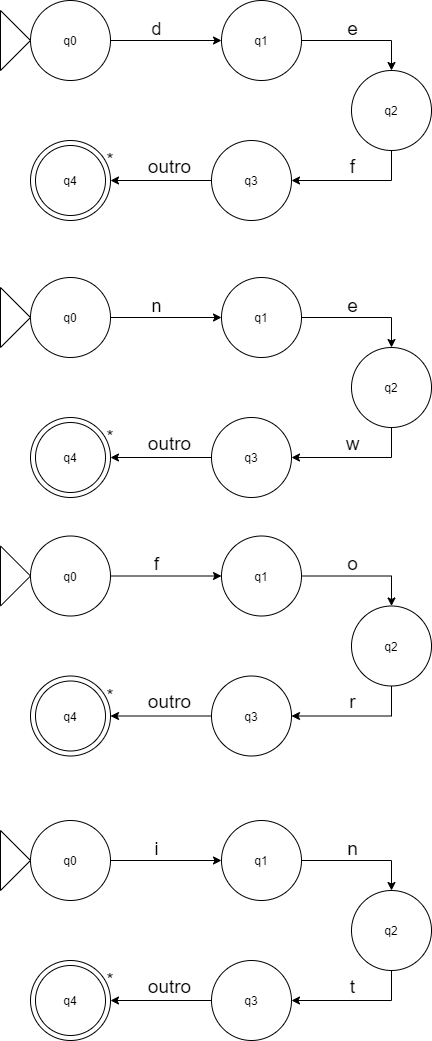
\includegraphics[scale=0.7]{6.png}
\\
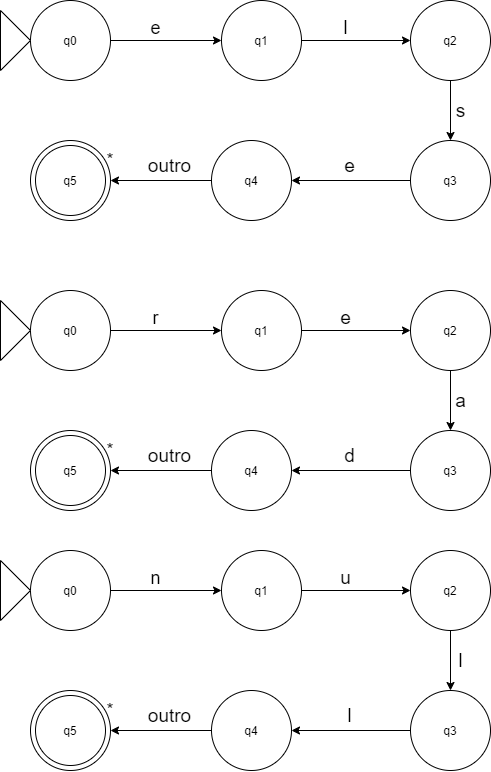
\includegraphics[scale=0.7]{7.png}
\\
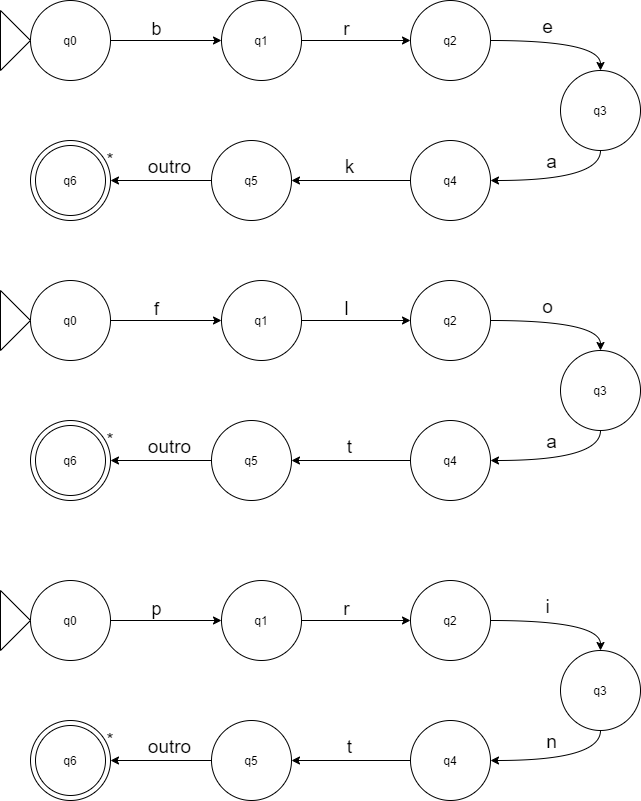
\includegraphics[scale=0.7]{8.png}
\\
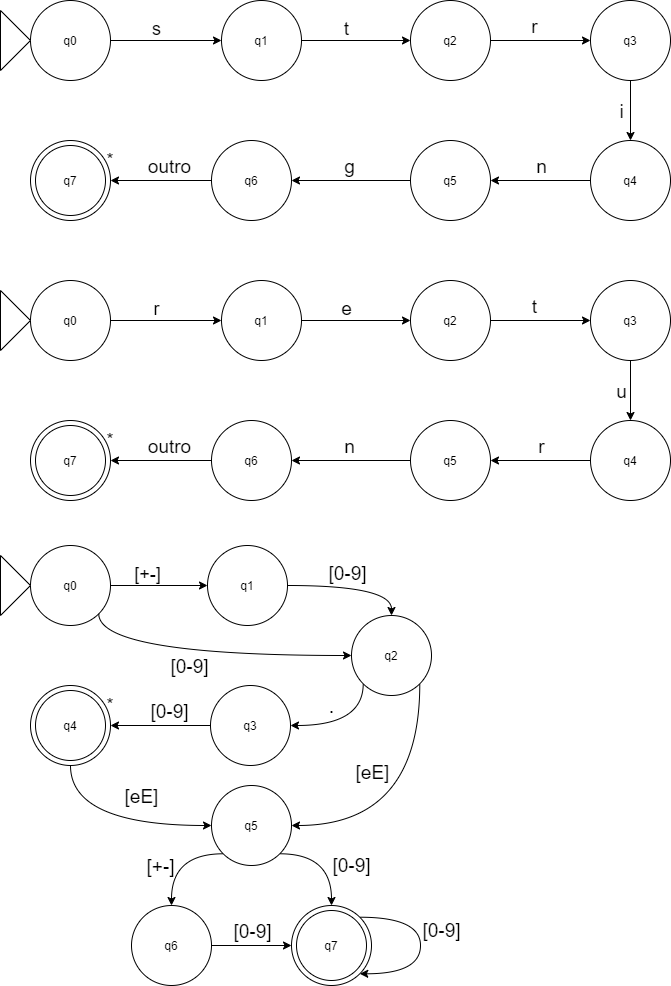
\includegraphics[scale=0.7]{9.png}

% ----------------------------------------------------------
% Finaliza a parte no bookmark do PDF
% para que se inicie o bookmark na raiz
% e adiciona espaço de parte no Sumário
% ----------------------------------------------------------
\phantompart
\part{Analisador Sintático}
\chapter{Ferramenta}
\section{Yacc}
O Yacc é uma abreviação do termo em inglês "\emph{Yet Another Compiler-Compiler}",
semelhante a ferramenta de mesmo nome para Unix. Ele é o componente do PLY que realiza
a análise da gramática.

Cada regra gramatical pode ser definida atravé de uma função Python, onde cada docstring possui
a especificação apropriada da gramática livre de contexto. Cada função aceita um
único argumento 'p', que é a sequência contendo os valores de cada símbolo da gramática
da respectiva regra. Segue um exemplo, de como especificamos a regra para a expressão \textbf{FUNCDEF}.

\begin{python}
def p_funcdef(p):
    '''
    funcdef : DEF IDENT LPAREN paramlist RPAREN LBRACE statelist RBRACE
    '''
\end{python}

Normalmente, a primeira regra especificada no yacc determina o começo da gramática.
Entretanto, podemos escolher qual regra da gramática o analisador deve iniciar
passando o parâmetro 'start=rule\_expression' para o yacc. No nosso trabalho,
ela pode ser representada pelas funções \emph{p\_program\_1}, \emph{p\_func\_list} ou
produções vazias e começa pela expressão \emph{program}. 

\begin{python}
def p_program_1(p):
    '''
    program : statement
    '''

def p_funclist(p):
    '''
    funclist : funcdef funclist1
    '''
    .
    .
    .
parser = yacc.yacc(start='program')  #build the parser
\end{python}

Para verificar problemas que ocorrem durante a análise sintática, podemos criar
uma regra para detectar erros sintáticos que são encontradas durante a análise. Além disso,
se algum erro é encontrado na especificação da gramática, o yacc irá produzir mensagems de 
diagnósticos ou exceções. Os problemas que podem ser encontrados são: funções com nomes duplicados,
conflitos gerados por gramáticas ambíguas, regras de gramáticas que são mal especificadas, recursões infinitas,
regras e tokens que não são utilizados ou definidos.

\begin{python}
def p_error(p):
    if not p:
        print("End of File!")
        return

    print("Erro:", p)
    print(text[p.lexpos - 40:p.lexpos + 40])   
\end{python} 


\chapter{Gramática}
\section{Gramática Original}

\begin{lstlisting}[escapechar=\#]
PROGRAM #$\rightarrow$# (STATEMENT | FUNCLIST)?

FUNCLIST #$\rightarrow$# FUNCDEF FUNCLIST | FUNCDEF  

FUNCDEF #$\rightarrow$# def ident(PARAMLIST){STATELIST}  

PARAMLIST #$\rightarrow$# ((int | float | string) ident, PARAMLIST |
             (int | float | string) ident)?  

STATEMENT #$\rightarrow$# (VARDECL; | ATRIBSTAT; | PRINTSTAT; |
             READSTAT; | RETURNSTAT; | IFSTAT | FORSTAT | {STATELIST} |
             break; | ;) 

VARDECL #$\rightarrow$# (int | float | string) ident ([int constant])#$^{*}$#

ATRIBSTAT #$\rightarrow$# LVALUE = (EXPRESSION | ALLOCEXPRESSION | FUNCCALL)

FUNCCALL #$\rightarrow$# ident(PARAMLISTCALL)  

PARAMLISTCALL #$\rightarrow$# (ident, PARAMLISTCALL | ident)?  

PRINTSTAT #$\rightarrow$# print EXPRESSION  

READSTAT #$\rightarrow$# read LVALUE  

RETURNSTAT #$\rightarrow$# return  

IFSTAT #$\rightarrow$# if(EXPRESSION ) STATEMENT (else STATEMENT)?  

FORSTAT #$\rightarrow$# for(ATRIBSTAT; EXPRESSION; ATRIBSTAT) STATEMENT  

STATELIST #$\rightarrow$# STATEMENT (STATELIST)?  

ALLOCEXPRESSION #$\rightarrow$# new (int | float | string) ([ NUMEXPRESSION ]) + 

EXPRESSION #$\rightarrow$# NUMEXPRESSION(( < | > | <= | >= | == | ! =) NUMEXPRESSION)? 

NUMEXPRESSION #$\rightarrow$# TERM ((+ | -) TERM)#$^{*}$#  

TERM #$\rightarrow$# UNARYEXPR(( * | / | %) UNARYEXPR)#$^{*}$#

UNARYEXPR #$\rightarrow$# ((+ | -))? FACTOR  

FACTOR #$\rightarrow$# (int_constant | float_constant | string_constant |
          null | LVALUE |(NUMEXPRESSION))  

LVALUE #$\rightarrow$# ident([NUMEXPRESSION])#$^{*}$# 
\end{lstlisting}

\section{Modificações na Gramática}
\begin{lstlisting}[escapechar=\#]
PROGRAM #$\rightarrow$# (STATEMENT | FUNCLIST)?  

FUNCLIST #$\rightarrow$# FUNCDEF FUNCLIST | FUNCDEF  

FUNCDEF #$\rightarrow$# def ident(PARAMLIST){STATELIST}  

PARAMLIST #$\rightarrow$# ((int | float | string)#$\textbf{\textcolor{red}{([])}}$##$^{*}$# ident, PARAMLIST |
             (int | float | string)#$\textbf{\textcolor{red}{([])}}$##$^{*}$# ident)?  

STATEMENT #$\rightarrow$# (VARDECL; | ATRIBSTAT; | PRINTSTAT; |
             READSTAT; | #$\textbf{\textcolor{red}{FUNCCALL;}}$#| RETURNSTAT; | IFSTAT | FORSTAT | #$\textbf{\textcolor{red}{WHILESTAT}}$# |
             {STATELIST} | break; | ;) 

VARDECL #$\rightarrow$# (int | float | string) ident ([int constant])#$^{*}$#  

ATRIBSTAT #$\rightarrow$# LVALUE#$\textbf{\textcolor{red}{([NUMEXPRESSION])?}}$# = (EXPRESSION |
             ALLOCEXPRESSION | FUNCCALL)  

FUNCCALL #$\rightarrow$# ident(PARAMLISTCALL)  

PARAMLISTCALL #$\rightarrow$# (ident#$\textbf{\textcolor{red}{([NUMEXPRESSION])}}$##$^{*}$#, PARAMLISTCALL | ident)?  

PRINTSTAT #$\rightarrow$# print EXPRESSION  

READSTAT #$\rightarrow$# read LVALUE  

RETURNSTAT #$\rightarrow$# return (#$\textbf{\textcolor{red}{ident | EXPRESSION)? }}$#

IFSTAT #$\rightarrow$# if(EXPRESSION ) STATEMENT (else STATEMENT)?  

FORSTAT #$\rightarrow$# for(ATRIBSTAT?; EXPRESSION?; ATRIBSTAT?) STATEMENT  

#$\textbf{\textcolor{red}{WHILESTAT}}$# #$\rightarrow$#  #$\textbf{\textcolor{red}{while(EXPRESSION) STATEMENT}}$#  

STATELIST #$\rightarrow$# STATEMENT (STATELIST)?  

ALLOCEXPRESSION #$\rightarrow$# new (int | float | string) ([NUMEXPRESSION]) +  

EXPRESSION #$\rightarrow$# NUMEXPRESSION(( < | > | <= | >= | == | ! =) NUMEXPRESSION)?  

NUMEXPRESSION #$\rightarrow$# TERM ((+ | -) TERM)#$^{*}$#  

TERM #$\rightarrow$# UNARYEXPR(( * | / | %) UNARYEXPR)#$^{*}$#  

UNARYEXPR #$\rightarrow$# ((+ | -))? FACTOR  

FACTOR #$\rightarrow$# (int_constant | float_constant | string_constant | null |
          LVALUE | (NUMEXPRESSION))  

LVALUE #$\rightarrow$# ident([NUMEXP RESSION])#$^{*}$# 
\end{lstlisting}

\section{Forma Convencional}
\subsection{Transformação para definição de gramática convencional}
\begin{lstlisting}[escapechar=\#]

PROGRAM #$\rightarrow$# STATEMENT | FUNCLIST | #$\bm{\varepsilon}$# 

FUNCLIST #$\rightarrow$# FUNCDEF FUNCLIST | FUNCDEF  

FUNCDEF #$\rightarrow$# def ident ( PARAMLIST ) { STATELIST }  

TYPES #$\rightarrow$#  int | float | string 

PARAMLIST #$\rightarrow$# TYPES LISTDCL_ident , PARAMLIST | TYPES LISTDCL ident | #$\bm{\varepsilon}$#  

LISTDCL #$\rightarrow$# []LISTDCL| #$\bm{\varepsilon}$# 

STATEMENT #$\rightarrow$# VARDECL ; |  ATRIBSTAT ; |  PRINTSTAT ; |
             READSTAT ;|  RETURNSTAT ; |  IFSTAT |  FORSTAT |  
             WHILESTAT |  { STATELIST } |  break; | ; 

VARDECL #$\rightarrow$# TYPES ident VARDECL' 

VARDECL' #$\rightarrow$#  [ int_constant ] VARDECL' | #$\bm{\varepsilon}$#  

ATRIBSTAT #$\rightarrow$# LVALUE ATRIBSTAT' = ATRIBSTAT'' 

ATRIBSTAT' #$\rightarrow$#  [ NUMEXPRESSION ] | #$\bm{\varepsilon}$#  

ATRIBSTAT'' #$\rightarrow$#  EXPRESSION | ALLOCEXPRESSION | FUNCCALL 

FUNCCALL #$\rightarrow$# ident ( PARAMLISTCALL )  

PARAMLISTCALL #$\rightarrow$# ident PARAMLISTCALL', PARAMLISTCALL | ident | #$\bm{\varepsilon}$#  

PARAMLISTCALL' #$\rightarrow$# [NUMEXPRESSION] | #$\bm{\varepsilon}$# 

PRINTSTAT #$\rightarrow$# print EXPRESSION  

READSTAT #$\rightarrow$# read LVALUE  

RETURNSTAT #$\rightarrow$# return RETURNSTAT' 

RETURNSTAT' #$\rightarrow$# ident | EXPRESSION | #$\bm{\varepsilon}$#  

IFSTAT #$\rightarrow$# if ( EXPRESSION ) STATEMENT IFSTAT'  

IFSTAT' #$\rightarrow$# else STATEMENT | #$\bm{\varepsilon}$#  

FORSTAT #$\rightarrow$# for ( FORSTAT' ; FORSTAT'' ; FORSTAT' ) STATEMENT  

FORSTAT' #$\rightarrow$# ATRIBSTAT | #$\bm{\varepsilon}$#  

FORSTAT'' #$\rightarrow$# EXPRESSION | #$\bm{\varepsilon}$#  

WHILESTAT #$\rightarrow$#  while ( EXPRESSION ) STATEMENT 

STATELIST #$\rightarrow$# STATEMENT STATELIST'  

STATELIST' #$\rightarrow$# STATELIST | #$\bm{\varepsilon}$#  

ALLOCEXPRESSION #$\rightarrow$# new TYPES [ NUMEXPRESSION ] ALLOCEXPRESSION' 

ALLOCEXPRESSION' #$\rightarrow$# [ NUMEXPRESSION ] ALLOCEXPRESSION' | #$\bm{\varepsilon}$#  

EXPRESSION #$\rightarrow$# NUMEXPRESSION EXPRESSION'  

EXPRESSION' #$\rightarrow$# COMPOPERATOR NUMEXPRESSION | #$\bm{\varepsilon}$#  

COMPOPERATOR #$\rightarrow$# < | > | < = | > = | = = | ! = 

NUMEXPRESSION #$\rightarrow$# TERM NUMEXPRESSION' 

NUMEXPRESSION' #$\rightarrow$# ADDSUB TERM | #$\bm{\varepsilon}$#  

ADDSUB #$\rightarrow$# + | - 

TERM #$\rightarrow$# UNARYEXPR TERM' 

TERM' #$\rightarrow$# MULTDIV UNARYEXPR TERM' | #$\bm{\varepsilon}$#   

MULTDIV #$\rightarrow$# * | / | %  

UNARYEXPR #$\rightarrow$# UNARYEXPR' FACTOR  

UNARYEXPR' #$\rightarrow$# ADDSUB | #$\bm{\varepsilon}$#  

FACTOR #$\rightarrow$# int_constant | float_constant | string_constant | null |
          LVALUE | ( NUMEXPRESSION ) 

LVALUE #$\rightarrow$# ident LVALUE' 

LVALUE' #$\rightarrow$# [ NUM_EXPRESSION ] LVALUE' | #$\bm{\varepsilon}$#  
\end{lstlisting}

\subsection{Remoção de recursão à esquerda}
\begin{lstlisting}[escapechar=\#]
PROGRAM #$\rightarrow$# STATEMENT | FUNCLIST | #$\bm{\varepsilon}$# 

FUNCLIST #$\rightarrow$# FUNCDEF FUNCLIST | FUNCDEF 

FUNCDEF #$\rightarrow$# def ident ( PARAMLIST ) { STATELIST } 

TYPES #$\rightarrow$# int | float | string 

PARAMLIST #$\rightarrow$# int LISTDCL ident , PARAMLIST 
             | float LISTDC ident , PARAMLIST 
             | string LISTDC ident , PARAMLIST 
             | int LISTDC ident  
             | float LISTDC ident 
             | string LISTDC ident 
             | #$\bm{\varepsilon}$# 

LISTDC #$\rightarrow$# []LISTDC | #$\bm{\varepsilon}$# 

STATEMENT #$\rightarrow$# VARDECL ; 
             | ATRIBSTAT ; 
             | PRINTSTAT ; 
             | READSTAT ; 
             | RETURNSTAT ; 
             | IFSTAT 
             | FORSTAT 
             | WHILESTAT 
             | { STATELIST } 
             | break ; 
             | ; 

VARDECL #$\rightarrow$# int ident VARDECL' 
           | float ident VARDECL' 
           | string ident VARDECL' 

VARDECL' #$\rightarrow$# [ int_constant ] VARDECL' 
            | #$\bm{\varepsilon}$# 

ATRIBSTAT #$\rightarrow$# LVALUE ATRIBSTAT' = ATRIBSTAT'' 

ATRIBSTAT' #$\rightarrow$# [ NUMEXPRESSION ] 
              | #$\bm{\varepsilon}$# 

ATRIBSTAT'' #$\rightarrow$# EXPRESSION 
               | ALLOCEXPRESSION 
               | FUNCCALL 

FUNCCALL #$\rightarrow$# ident ( PARAMLISTCALL ) 

PARAMLISTCALL #$\rightarrow$# ident PARAMLISTCALL', PARAMLISTCALL 
                 | ident PARAMLISTCALL'
                 | #$\bm{\varepsilon}$# 

PARAMLISTCALL' #$\rightarrow$# [NUMEXPRESSION] | #$\bm{\varepsilon}$#
PRINTSTAT #$\rightarrow$# print EXPRESSION 

READSTAT #$\rightarrow$# read LVALUE 

RETURNSTAT #$\rightarrow$# return RETURNSTAT' 

RETURNSTAT' #$\rightarrow$# ident 
               | EXPRESSION 
               | #$\bm{\varepsilon}$# 

IFSTAT #$\rightarrow$# if ( EXPRESSION ) STATEMENT IFSTAT' 

IFSTAT' #$\rightarrow$# else STATEMENT 
           | #$\bm{\varepsilon}$# 

FORSTAT #$\rightarrow$# for ( FORSTAT' ; FORSTAT'' ; FORSTAT' ) STATEMENT 

FORSTAT' #$\rightarrow$# LVALUE ATRIBSTAT' = ATRIBSTAT'' 
            | #$\bm{\varepsilon}$# 

FORSTAT'' #$\rightarrow$# EXPRESSION 
             | #$\bm{\varepsilon}$# 

WHILESTAT #$\rightarrow$# while ( EXPRESSION ) STATEMENT 

STATELIST #$\rightarrow$# int ident VARDECL' ; STATELIST' 
            | float ident VARDECL' ; STATELIST' 
            | string ident VARDECL' ; STATELIST' 
            | LVALUE ATRIBSTAT' = ATRIBSTAT'' ; STATELIST' 
            | print EXPRESSION ; STATELIST' 
            | read LVALUE ; STATELIST' 
            | return RETURNSTAT' ; STATELIST' 
            | if ( EXPRESSION ) STATEMENT IFSTAT' STATELIST' 
            | for ( FORSTAT' ; FORSTAT'' ; FORSTAT' ) STATEMENT STATELIST' 
            | while ( EXPRESSION ) STATEMENT STATELIST' 
            | { STATELIST } STATELIST' 
            | break ; STATELIST' 
            | ; STATELIST' 

STATELIST' #$\rightarrow$# int ident VARDECL' ; STATELIST' 
            | float ident VARDECL' ; STATELIST' 
            | string ident VARDECL' ; STATELIST' 
            | LVALUE ATRIBSTAT' = ATRIBSTAT'' ; STATELIST' 
            | print EXPRESSION ; STATELIST' 
            | read LVALUE ; STATELIST' 
            | return RETURNSTAT' ; STATELIST' 
            | if ( EXPRESSION ) STATEMENT IFSTAT' STATELIST' 
            | for ( FORSTAT' ; FORSTAT'' ; FORSTAT' ) STATEMENT STATELIST' 
            | while ( EXPRESSION ) STATEMENT STATELIST' 
            | { STATELIST } STATELIST' 
            | break ; STATELIST' 
            | ; STATELIST' 
            | #$\bm{\varepsilon}$# 

ALLOCEXPRESSION #$\rightarrow$# new TYPES [ NUMEXPRESSION ] ALLOCEXPRESSION' 

ALLOCEXPRESSION' #$\rightarrow$# [ NUMEXPRESSION ] ALLOCEXPRESSION' 
                    | #$\bm{\varepsilon}$# 

EXPRESSION #$\rightarrow$# NUMEXPRESSION EXPRESSION' 

EXPRESSION' #$\rightarrow$# COMPOPERATOR NUMEXPRESSION 
               | #$\bm{\varepsilon}$# 

COMPOPERATOR #$\rightarrow$# < 
              | > 
              | <= 
              | >= 
              | == 
              | !=  
NUMEXPRESSION #$\rightarrow$# TERM NUMEXPRESSION' 

NUMEXPRESSION' #$\rightarrow$# ADDSUB TERM 
                  | #$\bm{\varepsilon}$# 

ADDSUB #$\rightarrow$# + 
          | - 

TERM #$\rightarrow$# UNARYEXPR TERM' 

TERM' #$\rightarrow$# MULTDIV UNARYEXPR TERM' 
         | #$\bm{\varepsilon}$# 

MULTDIV #$\rightarrow$# * 
           | / 
           | % 

UNARYEXPR #$\rightarrow$# UNARYEXPR' FACTOR 

UNARYEXPR' #$\rightarrow$# + 
              | - 
              | #$\bm{\varepsilon}$# 

FACTOR #$\rightarrow$# int_constant 
          | float_constant 
          | string_constant 
          | null 
          | LVALUE 
          | ( NUMEXPRESSION ) 

LVALUE #$\rightarrow$# ident LVALUE' 

LVALUE' #$\rightarrow$# [ NUM_EXPRESSION ] LVALUE' 
           | #$\bm{\varepsilon}$# 
\end{lstlisting}

\subsection{Fatoração da Gramática}
\begin{lstlisting}[escapechar=\#]
PROGRAM #$\rightarrow$#  STATEMENT 
           | FUNCLIST 
           | #$\bm{\varepsilon}$# 

FUNCLIST #$\rightarrow$#  FUNCDEF FUNCLIST' 

FUNCLIST' #$\rightarrow$#  def ident ( PARAMLIST ) { STATELIST } FUNCLIST'
             | #$\bm{\varepsilon}$# 

FUNCDEF #$\rightarrow$#  def ident ( PARAMLIST ) { STATELIST } 

TYPES #$\rightarrow$#  int 
         | float 
         | string 

PARAMLIST #$\rightarrow$#  string LISTDCL ident PARAMLIST' 
             | float LISTDCL ident PARAMLIST' 
             | int LISTDCL ident PARAMLIST' 
             | #$\bm{\varepsilon}$# 

PARAMLIST' #$\rightarrow$# , PARAMLIST 
              | #$\bm{\varepsilon}$# 

LISTDCL #$\rightarrow$# []LISTDCL | #$\bm{\varepsilon}$# 

STATEMENT #$\rightarrow$#  VARDECL ; 
             | ATRIBSTAT ; 
             | PRINTSTAT ; 
             | READSTAT ; 
             | FUNCCALL ; 
             | RETURNSTAT ; 
             | IFSTAT 
             | FORSTAT 
             | WHILESTAT 
             | { STATELIST } 
             | break ; 
             | ; 

VARDECL #$\rightarrow$#  int ident VARDECL' 
           | float ident VARDECL' 
           | string ident VARDECL' 

VARDECL' #$\rightarrow$#  [ int_constant ] VARDECL' 
            | #$\bm{\varepsilon}$# 

ATRIBSTAT #$\rightarrow$#  LVALUE ATRIBSTAT' = ATRIBSTAT'' 

ATRIBSTAT' #$\rightarrow$#  [ NUMEXPRESSION ] 
              | #$\bm{\varepsilon}$# 

ATRIBSTAT'' #$\rightarrow$#  EXPRESSION 
               | ALLOCEXPRESSION 
               | FUNCCALL 

FUNCCALL #$\rightarrow$# ident ( PARAMLISTCALL ) 

PARAMLISTCALL #$\rightarrow$# ident PARAMLISTCALL' PARAMLISTCALL''
                 | #$\bm{\varepsilon}$# 

PARAMLISTCALL' #$\rightarrow$# [NUMEXPRESSION] | #$\bm{\varepsilon}$#                  

PARAMLISTCALL'' #$\rightarrow$#  , PARAMLISTCALL 
                  | #$\bm{\varepsilon}$# 

PRINTSTAT #$\rightarrow$#  print EXPRESSION 

READSTAT #$\rightarrow$#  read LVALUE 

RETURNSTAT #$\rightarrow$#  return RETURNSTAT' 

RETURNSTAT' #$\rightarrow$#  ident 
               | EXPRESSION 
               | #$\bm{\varepsilon}$# 

IFSTAT #$\rightarrow$#  if ( EXPRESSION ) STATEMENT IFSTAT' 

IFSTAT' #$\rightarrow$#  else STATEMENT 
           | #$\bm{\varepsilon}$# 

FORSTAT #$\rightarrow$#  for ( FORSTAT' ; FORSTAT'' ; FORSTAT' ) STATEMENT 

FORSTAT' #$\rightarrow$#  LVALUE ATRIBSTAT' = ATRIBSTAT'' 
            | #$\bm{\varepsilon}$# 

FORSTAT'' #$\rightarrow$#  EXPRESSION 
             | #$\bm{\varepsilon}$# 

WHILESTAT #$\rightarrow$#  while ( EXPRESSION ) STATEMENT 

STATELIST #$\rightarrow$#  int ident VARDECL' ; STATELIST' 
             | float ident VARDECL' ; STATELIST' 
             | string ident VARDECL' ; STATELIST' 
             | LVALUE ATRIBSTAT' = ATRIBSTAT'' ; STATELIST' 
             | print EXPRESSION ; STATELIST' 
             | read LVALUE ; STATELIST' 
             | ident ( PARAMLISTCALL ) ; STATELIST' 
             | return RETURNSTAT' ; STATELIST' 
             | if ( EXPRESSION ) STATEMENT IFSTAT' STATELIST' 
             | for ( FORSTAT' ; FORSTAT'' ; FORSTAT' ) STATEMENT STATELIST' 
             | while ( EXPRESSION ) STATEMENT STATELIST' 
             | { STATELIST } STATELIST' 
             | break ; STATELIST' 
             | ; STATELIST'

STATELIST' #$\rightarrow$#  int ident VARDECL' ; STATELIST' 
            | float ident VARDECL' ; STATELIST' 
            | string ident VARDECL' ; STATELIST' 
            | LVALUE ATRIBSTAT' = ATRIBSTAT'' ; STATELIST' 
            | print EXPRESSION ; STATELIST' 
            | read LVALUE ; STATELIST' 
            | ident ( PARAMLISTCALL ) ; STATELIST' 
            | return RETURNSTAT' ; STATELIST' 
            | if ( EXPRESSION ) STATEMENT IFSTAT' STATELIST' 
            | for ( FORSTAT' ; FORSTAT'' ; FORSTAT' ) STATEMENT STATELIST' 
            | while ( EXPRESSION ) STATEMENT STATELIST' 
            | { STATELIST } STATELIST' 
            | break ; STATELIST' 
            | ; STATELIST' 
            | #$\bm{\varepsilon}$# 

ALLOCEXPRESSION #$\rightarrow$#  new TYPES [ NUMEXPRESSION ] ALLOCEXPRESSION' 

ALLOCEXPRESSION' #$\rightarrow$#  [ NUMEXPRESSION ] ALLOCEXPRESSION' 
                  | #$\bm{\varepsilon}$# 

EXPRESSION #$\rightarrow$#  NUMEXPRESSION EXPRESSION' 

EXPRESSION' #$\rightarrow$#  COMPOPERATOR NUMEXPRESSION 
               | #$\bm{\varepsilon}$# 

COMPOPERATOR #$\rightarrow$#  < 
                | > 
                | <= 
                | >= 
                | == 
                | != 

NUMEXPRESSION #$\rightarrow$#  TERM NUMEXPRESSION' 

NUMEXPRESSION' #$\rightarrow$#  ADDSUB TERM 
                  | #$\bm{\varepsilon}$# 

ADDSUB #$\rightarrow$#  + 
          | - 

TERM #$\rightarrow$#  UNARYEXPR TERM' 

TERM' #$\rightarrow$#  MULTDIV UNARYEXPR TERM' 
         | #$\bm{\varepsilon}$# 

MULTDIV #$\rightarrow$#  * 
           | / 
           | % 

UNARYEXPR #$\rightarrow$#  UNARYEXPR' FACTOR 

UNARYEXPR' #$\rightarrow$#  + 
              | - 
              | #$\bm{\varepsilon}$# 

FACTOR #$\rightarrow$#  int_constant 
          | float_constant 
          | string_constant 
          | null 
          | LVALUE 
          | ( NUMEXPRESSION ) 

LVALUE #$\rightarrow$#  ident LVALUE' 

LVALUE' #$\rightarrow$#  [ NUM_EXPRESSION ] LVALUE' 
           | #$\bm{\varepsilon}$#    
           
\end{lstlisting}
% ---
% Conclusão (outro exemplo de capítulo sem numeração e presente no sumário)
% ---
\chapter*[Conclusão]{Conclusão}
Os compiladores traduzem o código fonte de uma linguagem de programação
de alto nível para uma linguagem de programação de baixo nível. Sem eles 
a tarefa de programar seria um trabalho extremamente lento e difícil.
São nichos específicos e muito raros os casos em que desenvolvemos
aplicações feitas diretamente em Assembly. Nos dias atuais, quase todas linguagens
possui o seu compilador, facilitando e aumentando a efetividade dos programadores.
Dito isto, com esse trabalho, foi possível entender a primeira parte da construção
de um compilador, ou seja, do analisador léxico. Utilizando a ferramenta PLY,
entendemos os princípios utilizados para se construir um compilador de uma
linguagem qualquer através da sua aplicação prática. Além disso, com o Diagrama
de Transição foi possível entender como ocorre a leitura das palavras e como são
identificado os tokens. Portanto, ao realizar este trabalho,
ficou evidente como criar um compilador através de ferramentas geradores de 
analisadores léxicos e sintáticos e dos estudos e pesquisas sobre compiladores.

\addcontentsline{toc}{chapter}{Conclusão}
% ---

% ----------------------------------------------------------
% ELEMENTOS PÓS-TEXTUAIS
% ----------------------------------------------------------
\postextual
% ----------------------------------------------------------

% ----------------------------------------------------------
% Referências bibliográficas
% ----------------------------------------------------------
\bibliography{abntex2-modelo-references}

% ----------------------------------------------------------
% Glossário
% ----------------------------------------------------------
%
% Consulte o manual da classe abntex2 para orientações sobre o glossário.
%
%\glossary

%---------------------------------------------------------------------
% INDICE REMISSIVO
%---------------------------------------------------------------------
\phantompart
\printindex
%---------------------------------------------------------------------

\end{document}